\PassOptionsToPackage{unicode=true}{hyperref} % options for packages loaded elsewhere
\PassOptionsToPackage{hyphens}{url}
%
\documentclass[
]{book}
\usepackage{lmodern}
\usepackage{amssymb,amsmath}
\usepackage{ifxetex,ifluatex}
\ifnum 0\ifxetex 1\fi\ifluatex 1\fi=0 % if pdftex
  \usepackage[T1]{fontenc}
  \usepackage[utf8]{inputenc}
  \usepackage{textcomp} % provides euro and other symbols
\else % if luatex or xelatex
  \usepackage{unicode-math}
  \defaultfontfeatures{Scale=MatchLowercase}
  \defaultfontfeatures[\rmfamily]{Ligatures=TeX,Scale=1}
\fi
% use upquote if available, for straight quotes in verbatim environments
\IfFileExists{upquote.sty}{\usepackage{upquote}}{}
\IfFileExists{microtype.sty}{% use microtype if available
  \usepackage[]{microtype}
  \UseMicrotypeSet[protrusion]{basicmath} % disable protrusion for tt fonts
}{}
\makeatletter
\@ifundefined{KOMAClassName}{% if non-KOMA class
  \IfFileExists{parskip.sty}{%
    \usepackage{parskip}
  }{% else
    \setlength{\parindent}{0pt}
    \setlength{\parskip}{6pt plus 2pt minus 1pt}}
}{% if KOMA class
  \KOMAoptions{parskip=half}}
\makeatother
\usepackage{xcolor}
\IfFileExists{xurl.sty}{\usepackage{xurl}}{} % add URL line breaks if available
\IfFileExists{bookmark.sty}{\usepackage{bookmark}}{\usepackage{hyperref}}
\hypersetup{
  pdftitle={R code demo for fast computing algorithm},
  pdfauthor={Shiqiang Jin and Gyuhyeong Goh},
  pdfborder={0 0 0},
  breaklinks=true}
\urlstyle{same}  % don't use monospace font for urls
\usepackage{color}
\usepackage{fancyvrb}
\newcommand{\VerbBar}{|}
\newcommand{\VERB}{\Verb[commandchars=\\\{\}]}
\DefineVerbatimEnvironment{Highlighting}{Verbatim}{commandchars=\\\{\}}
% Add ',fontsize=\small' for more characters per line
\usepackage{framed}
\definecolor{shadecolor}{RGB}{248,248,248}
\newenvironment{Shaded}{\begin{snugshade}}{\end{snugshade}}
\newcommand{\AlertTok}[1]{\textcolor[rgb]{0.94,0.16,0.16}{#1}}
\newcommand{\AnnotationTok}[1]{\textcolor[rgb]{0.56,0.35,0.01}{\textbf{\textit{#1}}}}
\newcommand{\AttributeTok}[1]{\textcolor[rgb]{0.77,0.63,0.00}{#1}}
\newcommand{\BaseNTok}[1]{\textcolor[rgb]{0.00,0.00,0.81}{#1}}
\newcommand{\BuiltInTok}[1]{#1}
\newcommand{\CharTok}[1]{\textcolor[rgb]{0.31,0.60,0.02}{#1}}
\newcommand{\CommentTok}[1]{\textcolor[rgb]{0.56,0.35,0.01}{\textit{#1}}}
\newcommand{\CommentVarTok}[1]{\textcolor[rgb]{0.56,0.35,0.01}{\textbf{\textit{#1}}}}
\newcommand{\ConstantTok}[1]{\textcolor[rgb]{0.00,0.00,0.00}{#1}}
\newcommand{\ControlFlowTok}[1]{\textcolor[rgb]{0.13,0.29,0.53}{\textbf{#1}}}
\newcommand{\DataTypeTok}[1]{\textcolor[rgb]{0.13,0.29,0.53}{#1}}
\newcommand{\DecValTok}[1]{\textcolor[rgb]{0.00,0.00,0.81}{#1}}
\newcommand{\DocumentationTok}[1]{\textcolor[rgb]{0.56,0.35,0.01}{\textbf{\textit{#1}}}}
\newcommand{\ErrorTok}[1]{\textcolor[rgb]{0.64,0.00,0.00}{\textbf{#1}}}
\newcommand{\ExtensionTok}[1]{#1}
\newcommand{\FloatTok}[1]{\textcolor[rgb]{0.00,0.00,0.81}{#1}}
\newcommand{\FunctionTok}[1]{\textcolor[rgb]{0.00,0.00,0.00}{#1}}
\newcommand{\ImportTok}[1]{#1}
\newcommand{\InformationTok}[1]{\textcolor[rgb]{0.56,0.35,0.01}{\textbf{\textit{#1}}}}
\newcommand{\KeywordTok}[1]{\textcolor[rgb]{0.13,0.29,0.53}{\textbf{#1}}}
\newcommand{\NormalTok}[1]{#1}
\newcommand{\OperatorTok}[1]{\textcolor[rgb]{0.81,0.36,0.00}{\textbf{#1}}}
\newcommand{\OtherTok}[1]{\textcolor[rgb]{0.56,0.35,0.01}{#1}}
\newcommand{\PreprocessorTok}[1]{\textcolor[rgb]{0.56,0.35,0.01}{\textit{#1}}}
\newcommand{\RegionMarkerTok}[1]{#1}
\newcommand{\SpecialCharTok}[1]{\textcolor[rgb]{0.00,0.00,0.00}{#1}}
\newcommand{\SpecialStringTok}[1]{\textcolor[rgb]{0.31,0.60,0.02}{#1}}
\newcommand{\StringTok}[1]{\textcolor[rgb]{0.31,0.60,0.02}{#1}}
\newcommand{\VariableTok}[1]{\textcolor[rgb]{0.00,0.00,0.00}{#1}}
\newcommand{\VerbatimStringTok}[1]{\textcolor[rgb]{0.31,0.60,0.02}{#1}}
\newcommand{\WarningTok}[1]{\textcolor[rgb]{0.56,0.35,0.01}{\textbf{\textit{#1}}}}
\usepackage{longtable,booktabs}
% Allow footnotes in longtable head/foot
\IfFileExists{footnotehyper.sty}{\usepackage{footnotehyper}}{\usepackage{footnote}}
\makesavenoteenv{longtable}
\usepackage{graphicx,grffile}
\makeatletter
\def\maxwidth{\ifdim\Gin@nat@width>\linewidth\linewidth\else\Gin@nat@width\fi}
\def\maxheight{\ifdim\Gin@nat@height>\textheight\textheight\else\Gin@nat@height\fi}
\makeatother
% Scale images if necessary, so that they will not overflow the page
% margins by default, and it is still possible to overwrite the defaults
% using explicit options in \includegraphics[width, height, ...]{}
\setkeys{Gin}{width=\maxwidth,height=\maxheight,keepaspectratio}
\setlength{\emergencystretch}{3em}  % prevent overfull lines
\providecommand{\tightlist}{%
  \setlength{\itemsep}{0pt}\setlength{\parskip}{0pt}}
\setcounter{secnumdepth}{5}
% Redefines (sub)paragraphs to behave more like sections
\ifx\paragraph\undefined\else
  \let\oldparagraph\paragraph
  \renewcommand{\paragraph}[1]{\oldparagraph{#1}\mbox{}}
\fi
\ifx\subparagraph\undefined\else
  \let\oldsubparagraph\subparagraph
  \renewcommand{\subparagraph}[1]{\oldsubparagraph{#1}\mbox{}}
\fi

% set default figure placement to htbp
\makeatletter
\def\fps@figure{htbp}
\makeatother

\usepackage{booktabs}
\usepackage[]{natbib}
\bibliographystyle{apalike}

\title{R code demo for fast computing algorithm}
\author{Shiqiang Jin and Gyuhyeong Goh}
\date{2020-06-22}

\begin{document}
\maketitle

{
\setcounter{tocdepth}{1}
\tableofcontents
}
\newcommand{\uA}{{\bf A}}
\newcommand{\ua}{{\bf a}}
\newcommand{\uB}{{\bf B}}
\newcommand{\ub}{{\bf b}}
\newcommand{\uC}{{\bf C}}
\newcommand{\uc}{{\bf c}}
\newcommand{\ud}{{\bf d}}
\newcommand{\ue}{{\bf e}}
\newcommand{\uE}{{\bf E}}
\newcommand{\uH}{{\bf H}}
\newcommand{\uI}{{\bf I}}
\newcommand{\uK}{{\bf K}}
\newcommand{\bP}{{\bf P}}
\newcommand{\uQ}{{\bf Q}}
\newcommand{\uv}{{\bf v}}
\newcommand{\uV}{{\bf V}}
\newcommand{\us}{{\bf s}}
\newcommand{\T}{{ \mathrm{\scriptscriptstyle T} }}
\newcommand{\uU}{{\bf U}}
\newcommand{\uu}{{\bf u}}
\newcommand{\uX}{{\bf X}}
\newcommand{\ux}{{\bf x}}
\newcommand{\uY}{{\bf Y}}
\newcommand{\uy}{{\bf y}}

\newcommand{\0}{{\bf 0}}
\newcommand{\1}{{\boldsymbol 1}}
\newcommand{\ualpha}{{\boldsymbol \alpha}}
\newcommand{\ubeta}{{\boldsymbol \beta}}
\newcommand{\diag}{{\rm diag}}
\newcommand{\uepsilon}{{\boldsymbol \epsilon}}
\newcommand{\ueta}{{\boldsymbol \eta}}
\newcommand{\bg}{{\boldsymbol \gamma}}
\newcommand{\bOmega}{{\boldsymbol\Omega}}
\newcommand{\uPsi}{{\boldsymbol \Psi}}
\newcommand{\uSigma}{{\boldsymbol \Sigma}}
\newcommand{\uxi}{{\boldsymbol \xi}}
\newcommand{\nbd}{{\text{nbd}}}

\hypertarget{r-code-demo-for-fast-computing-algorithm}{%
\chapter{R code demo for fast computing algorithm}\label{r-code-demo-for-fast-computing-algorithm}}

This is a supplymentary material about an R domo code for computing marginal likelihood distribution using fasting computing strategy and for-loop method

\hypertarget{review-of-appendix-b.1-calculation}{%
\section{Review of Appendix B.1 Calculation}\label{review-of-appendix-b.1-calculation}}

For any \(i\notin\hat{\boldsymbol \gamma}\), \(|\hat{\boldsymbol \gamma}\cup\{i\}|=k+1\), hence \(s({\bf Y}|\hat{\boldsymbol \gamma}\cup\{i\})\) in Eq.(3) can be expressed as
\begin{eqnarray}
s({\bf Y}|\hat{\boldsymbol \gamma}\cup\{i\})={\zeta}^{-\frac{m(k+1)}{2}}|{\bf X}_{\hat{\boldsymbol \gamma}\cup\{i\}}^{{ \mathrm{\scriptscriptstyle T} }}{\bf X}_{\hat{\boldsymbol \gamma}\cup\{i\}}+\zeta^{-1}{\bf I}_{k+1}|^{-\frac{m}{2}}| {\bf Y}^{{ \mathrm{\scriptscriptstyle T} }}{\bf H}_{\hat{\boldsymbol \gamma}\cup\{i\}}{\bf Y}+{\boldsymbol \Psi}|^{-\frac{n+\nu}{2}}.
\label{eq:1}
\end{eqnarray}

Using technique fast computing algorithm, we have

\begin{eqnarray}
{\bf s}_+(\hat{\boldsymbol \gamma}) &=& c_{\hat{\boldsymbol \gamma}}^+\times \left(\zeta^{-1}{\boldsymbol 1}_p+{\rm diag}({\bf X}^{{ \mathrm{\scriptscriptstyle T} }}{\bf H}_{\hat{{\boldsymbol \gamma}}}{\bf X})\right)^{-m/2}\boldsymbol{\cdot}\\
&&\left[{\boldsymbol 1}_p - \frac{{\rm diag}({\bf X}^{{ \mathrm{\scriptscriptstyle T} }}{\bf H}_{\hat{{\boldsymbol \gamma}}}{\bf Y}({\bf Y}^{{ \mathrm{\scriptscriptstyle T} }}{\bf H}_{\hat{{\boldsymbol \gamma}}}{\bf Y}+{\boldsymbol \Psi})^{-1}{\bf Y}^{{ \mathrm{\scriptscriptstyle T} }}{\bf H}_{\hat{{\boldsymbol \gamma}}}{\bf X})}{\zeta^{-1}{\boldsymbol 1}_p+{\rm diag}({\bf X}^{{ \mathrm{\scriptscriptstyle T} }}{\bf H}_{\hat{{\boldsymbol \gamma}}}{\bf X})}\right]^{-\frac{n+\nu}{2}}\label{eq:2}
\end{eqnarray}
where \({\bf a}^x = (a_1^x,\ldots,a_p^x)\), \({\bf a}\boldsymbol{\cdot}{\bf b}= (a_1b_1,\ldots,a_pb_p)\), \({\bf a}/{\bf b}= (a_1/b_1,\ldots,a_p/b_p)\) for generic vectors \({\bf a}\) and \({\bf b}\), and \(c_{\hat{\boldsymbol \gamma}}^+= {\zeta}^{-\frac{m(k+1)}{2}}|{\bf X}_{\hat{\boldsymbol \gamma}}^{{ \mathrm{\scriptscriptstyle T} }}{\bf X}_{\hat{\boldsymbol \gamma}}+\zeta^{-1}{\bf I}_{k}|^{-\frac{m}{2}}\left|{\bf Y}^{{ \mathrm{\scriptscriptstyle T} }}{\bf H}_{\hat{{\boldsymbol \gamma}}}{\bf Y}+{\boldsymbol \Psi}\right|^{-\frac{n+\nu}{2}}\) is a constant with respect to \(i\notin \hat{\boldsymbol \gamma}\).

Hence,
\begin{eqnarray}
\log({\bf s}_+(\hat{\boldsymbol \gamma})) = \log(c_{\hat{\boldsymbol \gamma}}^+){\boldsymbol 1}_p-\frac{m}{2}\log({\bf d})-\frac{n+\nu}{2}\log(1-\frac{{\bf u}}{{\bf d}}),\label{eq:3}
\end{eqnarray}
where \({\bf d}= \zeta^{-1}{\boldsymbol 1}_p+{\rm diag}({\bf X}^{{ \mathrm{\scriptscriptstyle T} }}{\bf H}_{\hat{{\boldsymbol \gamma}}}{\bf X})\) and \({\bf u}={\rm diag}({\bf X}^{{ \mathrm{\scriptscriptstyle T} }}{\bf H}_{\hat{{\boldsymbol \gamma}}}{\bf Y}({\bf Y}^{{ \mathrm{\scriptscriptstyle T} }}{\bf H}_{\hat{{\boldsymbol \gamma}}}{\bf Y}+{\boldsymbol \Psi})^{-1}{\bf Y}^{{ \mathrm{\scriptscriptstyle T} }}{\bf H}_{\hat{{\boldsymbol \gamma}}}{\bf X})\).

In the following simulation example, I will evaluate \({\bf s}({\bf Y}|{\text{nbd}}_+(\hat{\boldsymbol \gamma}))\) by \eqref{eq:1} in the ``for-loop'' method and by \eqref{eq:3} in a single calculation.

\hypertarget{simulation-example}{%
\section{Simulation example}\label{simulation-example}}

In this example, we

\begin{itemize}
\tightlist
\item
  specify the model setting as \(n=100, p = 1000, m = 5, \zeta = \log(n), {\boldsymbol \Psi}= 0.5{\bf I}_m, \nu = 0.5\).
\end{itemize}

\begin{Shaded}
\begin{Highlighting}[]
\NormalTok{n <-}\StringTok{ }\DecValTok{100}
\NormalTok{p <-}\StringTok{ }\DecValTok{1000}
\NormalTok{m <-}\StringTok{ }\DecValTok{5}
\NormalTok{zeta <-}\StringTok{ }\KeywordTok{log}\NormalTok{(n)}
\NormalTok{Psi <-}\StringTok{ }\KeywordTok{diag}\NormalTok{(}\FloatTok{0.5}\NormalTok{, m)  }\CommentTok{# Psi}
\NormalTok{v <-}\StringTok{ }\FloatTok{0.5}  \CommentTok{# nu}
\end{Highlighting}
\end{Shaded}

\begin{itemize}
\tightlist
\item
  and generate data \({\bf Y}={\bf X}{\bf C}+ {\bf E}\) with \({\bf E}\sim \mathcal{N}(0, {\boldsymbol\Omega})\); The true model is \({\boldsymbol \gamma}^* = (1,2,3,4,7,8,9,10)\) and the current model \(\hat{\boldsymbol \gamma}= (1,2,3,4,7,8,9)\) with model size \(|\hat{\boldsymbol \gamma}| = 7\). \({\boldsymbol\Omega}= 0.2^{|i-j|}\) and \({\bf X}\) is generated from \(\mathcal{N}({\bf 0}, {\boldsymbol \Sigma})\) with \({\boldsymbol \Sigma}= 0.2^{|i-j|}\).
\end{itemize}

\begin{Shaded}
\begin{Highlighting}[]
\CommentTok{# Generate data}
\KeywordTok{library}\NormalTok{(mvtnorm)}
\KeywordTok{set.seed}\NormalTok{(}\DecValTok{1314}\NormalTok{)}
\NormalTok{true.model <-}\StringTok{ }\KeywordTok{c}\NormalTok{(}\DecValTok{1}\OperatorTok{:}\DecValTok{4}\NormalTok{, }\DecValTok{7}\OperatorTok{:}\DecValTok{10}\NormalTok{)  }\CommentTok{# true model}
\NormalTok{r <-}\StringTok{ }\KeywordTok{c}\NormalTok{(}\DecValTok{1}\OperatorTok{:}\DecValTok{4}\NormalTok{, }\DecValTok{7}\OperatorTok{:}\DecValTok{9}\NormalTok{)  }\CommentTok{# current model}
\NormalTok{k <-}\StringTok{ }\KeywordTok{length}\NormalTok{(r)  }\CommentTok{# current model size}
\NormalTok{rho_e <-}\StringTok{ }\FloatTok{0.2}
\NormalTok{Omega <-}\StringTok{ }\NormalTok{rho_e}\OperatorTok{^}\NormalTok{(}\KeywordTok{abs}\NormalTok{(}\KeywordTok{matrix}\NormalTok{(}\DecValTok{1}\OperatorTok{:}\NormalTok{m, m, m) }\OperatorTok{-}\StringTok{ }\KeywordTok{t}\NormalTok{(}\KeywordTok{matrix}\NormalTok{(}\DecValTok{1}\OperatorTok{:}\NormalTok{m, m, m))))}
\NormalTok{rho_x <-}\StringTok{ }\FloatTok{0.2}
\NormalTok{Sig_x <-}\StringTok{ }\NormalTok{rho_x}\OperatorTok{^}\NormalTok{(}\KeywordTok{abs}\NormalTok{(}\KeywordTok{matrix}\NormalTok{(}\DecValTok{1}\OperatorTok{:}\NormalTok{p, p, p) }\OperatorTok{-}\StringTok{ }\KeywordTok{t}\NormalTok{(}\KeywordTok{matrix}\NormalTok{(}\DecValTok{1}\OperatorTok{:}\NormalTok{p, p, p))))}
\NormalTok{seq.p <-}\StringTok{ }\KeywordTok{c}\NormalTok{(}\DecValTok{1}\OperatorTok{:}\NormalTok{p)}
\NormalTok{len.true.model <-}\StringTok{ }\KeywordTok{length}\NormalTok{(true.model)}
\CommentTok{# generate random coefficient matrix C}
\NormalTok{c0 <-}\StringTok{ }\KeywordTok{sample}\NormalTok{(}\KeywordTok{seq}\NormalTok{(}\OperatorTok{-}\DecValTok{1}\NormalTok{, }\DecValTok{1}\NormalTok{, }\FloatTok{0.2}\NormalTok{), }\DataTypeTok{size =}\NormalTok{ len.true.model }\OperatorTok{*}\StringTok{ }\NormalTok{m, }\DataTypeTok{replace =} \OtherTok{TRUE}\NormalTok{)}
\NormalTok{C <-}\StringTok{ }\KeywordTok{matrix}\NormalTok{(}\DecValTok{0}\NormalTok{, p, m)}
\NormalTok{C[true.model, ] <-}\StringTok{ }\KeywordTok{matrix}\NormalTok{(c0, len.true.model, m)}
\NormalTok{X <-}\StringTok{ }\KeywordTok{rmvnorm}\NormalTok{(n, }\KeywordTok{rep}\NormalTok{(}\DecValTok{0}\NormalTok{, p), Sig_x, }\DataTypeTok{method =} \StringTok{"chol"}\NormalTok{)}
\NormalTok{E <-}\StringTok{ }\KeywordTok{rmvnorm}\NormalTok{(n, }\DataTypeTok{mean =} \KeywordTok{rep}\NormalTok{(}\DecValTok{0}\NormalTok{, m), }\DataTypeTok{sigma =}\NormalTok{ Omega)}
\NormalTok{Y <-}\StringTok{ }\KeywordTok{as.numeric}\NormalTok{(X }\OperatorTok\StringTok{ }\NormalTok{C) }\OperatorTok{+}\StringTok{ }\NormalTok{E}
\end{Highlighting}
\end{Shaded}

To better understand R code and corresponding notations, we list a cross-reference table for some of them as follows:

\begin{longtable}[]{@{}cccccc@{}}
\toprule
\endhead
\begin{minipage}[t]{0.14\columnwidth}\centering
I\_n\strut
\end{minipage} & \begin{minipage}[t]{0.14\columnwidth}\centering
I\_k1\strut
\end{minipage} & \begin{minipage}[t]{0.14\columnwidth}\centering
log.s.plus1 or log.s.plus2\strut
\end{minipage} & \begin{minipage}[t]{0.14\columnwidth}\centering
rUi\strut
\end{minipage} & \begin{minipage}[t]{0.14\columnwidth}\centering
X.rUi\strut
\end{minipage} & \begin{minipage}[t]{0.14\columnwidth}\centering
H.rUi\strut
\end{minipage}\tabularnewline
\begin{minipage}[t]{0.14\columnwidth}\centering
\({\bf I}_n\)\strut
\end{minipage} & \begin{minipage}[t]{0.14\columnwidth}\centering
\({\bf I}_{k+1}\)\strut
\end{minipage} & \begin{minipage}[t]{0.14\columnwidth}\centering
\(\log({\bf s}({\bf Y}|{\text{nbd}}_+(\hat{\boldsymbol \gamma})))\)\strut
\end{minipage} & \begin{minipage}[t]{0.14\columnwidth}\centering
\(\hat{\boldsymbol \gamma}\cup i\)\strut
\end{minipage} & \begin{minipage}[t]{0.14\columnwidth}\centering
\({\bf X}_{\hat{\boldsymbol \gamma}\cup i}\)\strut
\end{minipage} & \begin{minipage}[t]{0.14\columnwidth}\centering
\({\bf H}_{\hat{\boldsymbol \gamma}\cup i}\)\strut
\end{minipage}\tabularnewline
\begin{minipage}[t]{0.14\columnwidth}\centering
log.s.Y.rUi\strut
\end{minipage} & \begin{minipage}[t]{0.14\columnwidth}\centering
I\_k\strut
\end{minipage} & \begin{minipage}[t]{0.14\columnwidth}\centering
X.r\strut
\end{minipage} & \begin{minipage}[t]{0.14\columnwidth}\centering
X\_r\strut
\end{minipage} & \begin{minipage}[t]{0.14\columnwidth}\centering
H.r\strut
\end{minipage} & \begin{minipage}[t]{0.14\columnwidth}\centering
colSums(H.r\%*\%X\_r*X\_r)\strut
\end{minipage}\tabularnewline
\begin{minipage}[t]{0.14\columnwidth}\centering
\(\log(s({\bf Y}|\hat{\boldsymbol \gamma}\cup i))\)\strut
\end{minipage} & \begin{minipage}[t]{0.14\columnwidth}\centering
\({\bf I}_k\)\strut
\end{minipage} & \begin{minipage}[t]{0.14\columnwidth}\centering
\({\bf X}_{\hat{\boldsymbol \gamma}}\)\strut
\end{minipage} & \begin{minipage}[t]{0.14\columnwidth}\centering
\({\bf X}_{-\hat{\boldsymbol \gamma}}\)\strut
\end{minipage} & \begin{minipage}[t]{0.14\columnwidth}\centering
\({\bf H}_{\hat{\boldsymbol \gamma}}\)\strut
\end{minipage} & \begin{minipage}[t]{0.14\columnwidth}\centering
\({\rm diag}({\bf X}_{-\hat{\boldsymbol \gamma}}^{{ \mathrm{\scriptscriptstyle T} }}{\bf H}_{\hat{{\boldsymbol \gamma}}}{\bf X}_{-\hat{\boldsymbol \gamma}})\)\strut
\end{minipage}\tabularnewline
\begin{minipage}[t]{0.14\columnwidth}\centering
YHX\_r\strut
\end{minipage} & \begin{minipage}[t]{0.14\columnwidth}\centering
\strut
\end{minipage} & \begin{minipage}[t]{0.14\columnwidth}\centering
\strut
\end{minipage} & \begin{minipage}[t]{0.14\columnwidth}\centering
\strut
\end{minipage} & \begin{minipage}[t]{0.14\columnwidth}\centering
\strut
\end{minipage} & \begin{minipage}[t]{0.14\columnwidth}\centering
\strut
\end{minipage}\tabularnewline
\begin{minipage}[t]{0.14\columnwidth}\centering
\({\bf Y}^{{ \mathrm{\scriptscriptstyle T} }}{\bf H}_{\hat{{\boldsymbol \gamma}}}{\bf X}_{-\hat{\boldsymbol \gamma}}\)\strut
\end{minipage} & \begin{minipage}[t]{0.14\columnwidth}\centering
\strut
\end{minipage} & \begin{minipage}[t]{0.14\columnwidth}\centering
\strut
\end{minipage} & \begin{minipage}[t]{0.14\columnwidth}\centering
\strut
\end{minipage} & \begin{minipage}[t]{0.14\columnwidth}\centering
\strut
\end{minipage} & \begin{minipage}[t]{0.14\columnwidth}\centering
\strut
\end{minipage}\tabularnewline
\bottomrule
\end{longtable}

\begin{Shaded}
\begin{Highlighting}[]
\CommentTok{# For loop method}
\NormalTok{I_n <-}\StringTok{ }\KeywordTok{diag}\NormalTok{(}\DecValTok{1}\NormalTok{, n)  }\CommentTok{# n-dimension identity matrix }
\NormalTok{I_k1 <-}\StringTok{ }\KeywordTok{diag}\NormalTok{(}\DecValTok{1}\NormalTok{, k }\OperatorTok{+}\StringTok{ }\DecValTok{1}\NormalTok{)}
\NormalTok{p_r <-}\StringTok{ }\KeywordTok{setdiff}\NormalTok{(}\KeywordTok{seq}\NormalTok{(}\DecValTok{1}\NormalTok{, p), r)  }\CommentTok{# p-k vector}
\NormalTok{log.s.plus1 <-}\StringTok{ }\KeywordTok{rep}\NormalTok{(}\OtherTok{NA}\NormalTok{, }\KeywordTok{length}\NormalTok{(p_r))}
\NormalTok{j <-}\StringTok{ }\DecValTok{1}
\ControlFlowTok{for}\NormalTok{ (i }\ControlFlowTok{in}\NormalTok{ p_r) \{}
\NormalTok{    rUi <-}\StringTok{ }\KeywordTok{sort}\NormalTok{(}\KeywordTok{c}\NormalTok{(r, i))  }\CommentTok{# add one index from p_r}
\NormalTok{    X.rUi <-}\StringTok{ }\NormalTok{X[, rUi]  }\CommentTok{# model in addition neighbor}
\NormalTok{    XtX <-}\StringTok{ }\KeywordTok{crossprod}\NormalTok{(X.rUi) }\OperatorTok{+}\StringTok{ }\DecValTok{1}\OperatorTok{/}\NormalTok{zeta }\OperatorTok{*}\StringTok{ }\NormalTok{I_k1}
\NormalTok{    H.rUi <-}\StringTok{ }\NormalTok{I_n }\OperatorTok{-}\StringTok{ }\NormalTok{X.rUi }\OperatorTok\StringTok{ }\KeywordTok{solve}\NormalTok{(XtX) }\OperatorTok\StringTok{ }\KeywordTok{t}\NormalTok{(X.rUi)}
    \CommentTok{# logarithm of Eq (1.1)}
\NormalTok{    log.s.Y.rUi <-}\StringTok{ }\OperatorTok{-}\NormalTok{m }\OperatorTok{*}\StringTok{ }\NormalTok{(k }\OperatorTok{+}\StringTok{ }\DecValTok{1}\NormalTok{)}\OperatorTok{/}\DecValTok{2} \OperatorTok{*}\StringTok{ }\KeywordTok{log}\NormalTok{(zeta) }\OperatorTok{-}\StringTok{ }\NormalTok{m}\OperatorTok{/}\DecValTok{2} \OperatorTok{*}\StringTok{ }\KeywordTok{log}\NormalTok{(}\KeywordTok{det}\NormalTok{(XtX)) }\OperatorTok{-}\StringTok{ }\NormalTok{(n }\OperatorTok{+}\StringTok{ }\NormalTok{v)}\OperatorTok{/}\DecValTok{2} \OperatorTok{*}\StringTok{ }\KeywordTok{log}\NormalTok{(}\KeywordTok{det}\NormalTok{(}\KeywordTok{t}\NormalTok{(Y) }\OperatorTok\StringTok{ }\NormalTok{H.rUi }\OperatorTok\StringTok{ }\NormalTok{Y }\OperatorTok{+}\StringTok{ }\NormalTok{Psi))}
\NormalTok{    log.s.plus1[j] <-}\StringTok{ }\NormalTok{log.s.Y.rUi}
\NormalTok{    j <-}\StringTok{ }\NormalTok{j }\OperatorTok{+}\StringTok{ }\DecValTok{1}
\NormalTok{\}}

\CommentTok{# Proposed Method}
\NormalTok{I_k <-}\StringTok{ }\KeywordTok{diag}\NormalTok{(}\DecValTok{1}\NormalTok{, k)  }\CommentTok{# k-dimension identity matrix }
\NormalTok{X.r <-}\StringTok{ }\NormalTok{X[, r]}
\NormalTok{X_r <-}\StringTok{ }\NormalTok{X[, p_r]  }\CommentTok{# n by p-k m sub-matrix of X}
\NormalTok{H.r <-}\StringTok{ }\NormalTok{I_n }\OperatorTok{-}\StringTok{ }\NormalTok{X.r }\OperatorTok\StringTok{ }\KeywordTok{solve}\NormalTok{(}\KeywordTok{crossprod}\NormalTok{(X.r) }\OperatorTok{+}\StringTok{ }\DecValTok{1}\OperatorTok{/}\NormalTok{zeta }\OperatorTok{*}\StringTok{ }\NormalTok{I_k) }\OperatorTok\StringTok{ }\KeywordTok{t}\NormalTok{(X.r)  }\CommentTok{# n by n matrix}
\NormalTok{d <-}\StringTok{ }\DecValTok{1}\OperatorTok{/}\NormalTok{zeta }\OperatorTok{+}\StringTok{ }\KeywordTok{colSums}\NormalTok{(H.r }\OperatorTok\StringTok{ }\NormalTok{X_r }\OperatorTok{*}\StringTok{ }\NormalTok{X_r)  }\CommentTok{# p-k dimension vector}
\NormalTok{YHX_r <-}\StringTok{ }\KeywordTok{t}\NormalTok{(Y) }\OperatorTok\StringTok{ }\NormalTok{H.r }\OperatorTok\StringTok{ }\NormalTok{X_r  }\CommentTok{# p-k by m matrix}
\NormalTok{YHY_}\DecValTok{1}\NormalTok{ <-}\StringTok{ }\KeywordTok{solve}\NormalTok{(}\KeywordTok{t}\NormalTok{(Y) }\OperatorTok\StringTok{ }\NormalTok{H.r }\OperatorTok\StringTok{ }\NormalTok{Y }\OperatorTok{+}\StringTok{ }\NormalTok{Psi)  }\CommentTok{# m by m matrix}
\NormalTok{u <-}\StringTok{ }\KeywordTok{colSums}\NormalTok{(YHY_}\DecValTok{1} \OperatorTok\StringTok{ }\NormalTok{YHX_r }\OperatorTok{*}\StringTok{ }\NormalTok{YHX_r)  }\CommentTok{# p-k dimension vector}

\CommentTok{# logarithm of Eq (1.3)}
\NormalTok{log.s.plus1.approx <-}\StringTok{ }\OperatorTok{-}\NormalTok{m}\OperatorTok{/}\DecValTok{2} \OperatorTok{*}\StringTok{ }\KeywordTok{log}\NormalTok{(d) }\OperatorTok{-}\StringTok{ }\NormalTok{(n }\OperatorTok{+}\StringTok{ }\NormalTok{v)}\OperatorTok{/}\DecValTok{2} \OperatorTok{*}\StringTok{ }\KeywordTok{log}\NormalTok{(}\DecValTok{1} \OperatorTok{-}\StringTok{ }\NormalTok{u}\OperatorTok{/}\NormalTok{d)}
\CommentTok{# log(c)}
\NormalTok{log.c <-}\StringTok{ }\FloatTok{-0.5} \OperatorTok{*}\StringTok{ }\NormalTok{m }\OperatorTok{*}\StringTok{ }\NormalTok{(k }\OperatorTok{+}\StringTok{ }\DecValTok{1}\NormalTok{) }\OperatorTok{*}\StringTok{ }\KeywordTok{log}\NormalTok{(zeta) }\OperatorTok{-}\StringTok{ }\FloatTok{0.5} \OperatorTok{*}\StringTok{ }\NormalTok{m }\OperatorTok{*}\StringTok{ }\KeywordTok{log}\NormalTok{(}\KeywordTok{det}\NormalTok{(}\KeywordTok{crossprod}\NormalTok{(X.r) }\OperatorTok{+}\StringTok{ }
\StringTok{    }\DecValTok{1}\OperatorTok{/}\NormalTok{zeta }\OperatorTok{*}\StringTok{ }\NormalTok{I_k)) }\OperatorTok{-}\StringTok{ }\NormalTok{(n }\OperatorTok{+}\StringTok{ }\NormalTok{v)}\OperatorTok{/}\DecValTok{2} \OperatorTok{*}\StringTok{ }\KeywordTok{log}\NormalTok{(}\KeywordTok{det}\NormalTok{(}\KeywordTok{t}\NormalTok{(Y) }\OperatorTok\StringTok{ }\NormalTok{H.r }\OperatorTok\StringTok{ }\NormalTok{Y }\OperatorTok{+}\StringTok{ }\NormalTok{Psi))}
\NormalTok{log.s.plus2 <-}\StringTok{ }\NormalTok{log.c }\OperatorTok{+}\StringTok{ }\NormalTok{log.s.plus1.approx  }\CommentTok{# logarithm of Eq (1.2)}
\end{Highlighting}
\end{Shaded}

I compute mean absolute percentage error \(\text{MAPE} = \frac{1}{n}\Sigma_{t=1}^n|\frac{A_t-F_t}{A_t}|\) to measure the accuracy of the fast computing algorithm.

\begin{Shaded}
\begin{Highlighting}[]
\CommentTok{# Mean absolute percentage error}
\NormalTok{MAPE <-}\StringTok{ }\KeywordTok{mean}\NormalTok{(}\KeywordTok{abs}\NormalTok{(log.s.plus1 }\OperatorTok{-}\StringTok{ }\NormalTok{log.s.plus2)}\OperatorTok{/}\KeywordTok{abs}\NormalTok{(log.s.plus1))}
\KeywordTok{print}\NormalTok{(}\KeywordTok{paste}\NormalTok{(}\StringTok{"MAPE ="}\NormalTok{, MAPE))}
\end{Highlighting}
\end{Shaded}

\begin{verbatim}
## [1] "MAPE = 8.12298413315687e-17"
\end{verbatim}

\begin{Shaded}
\begin{Highlighting}[]
\KeywordTok{plot}\NormalTok{(log.s.plus1, log.s.plus2)}
\KeywordTok{abline}\NormalTok{(}\DataTypeTok{a =} \DecValTok{0}\NormalTok{, }\DataTypeTok{b =} \DecValTok{1}\NormalTok{)}
\end{Highlighting}
\end{Shaded}

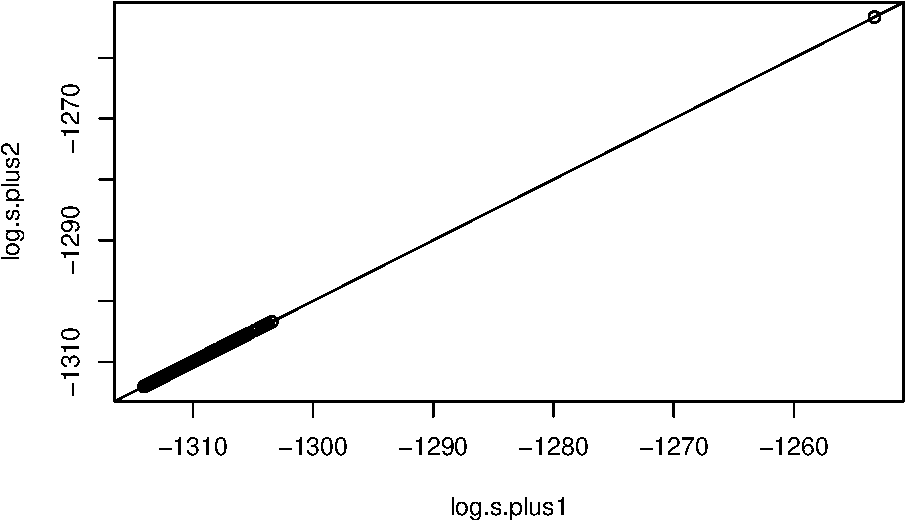
\includegraphics{RdemoMVRM_files/figure-latex/unnamed-chunk-4-1.pdf}

From the plot and MAPE, \(\log({\bf s}({\bf Y}|{\text{nbd}}_+(\hat{\boldsymbol \gamma})))\) computed by \eqref{eq:1} and \eqref{eq:3} are the same. But the time costs are different.

\hypertarget{time-cost-comparison-for-proposed-method-and-for-loop-method}{%
\section{Time cost comparison for proposed method and for loop method}\label{time-cost-comparison-for-proposed-method-and-for-loop-method}}

Note that when doing the model selection, as \(\log(c_{\hat{\boldsymbol \gamma}}^+)\) is a constant with respect to \(i\notin \hat{\boldsymbol \gamma}\), in R code I only compute \texttt{log.s.plus2.approx}. I use R package \texttt{microbenchmark} to do the simulation and the default replication is 100 times.

\begin{Shaded}
\begin{Highlighting}[]
\KeywordTok{library}\NormalTok{(microbenchmark)}
\NormalTok{timecost <-}\StringTok{ }\KeywordTok{microbenchmark}\NormalTok{(}\StringTok{"for_loop"}\NormalTok{ =}\StringTok{ }\NormalTok{\{}
\NormalTok{  log.s.plus1 <-}\StringTok{ }\KeywordTok{rep}\NormalTok{(}\OtherTok{NA}\NormalTok{, }\KeywordTok{length}\NormalTok{(p_r))}
\NormalTok{  j <-}\StringTok{ }\DecValTok{1}
  \ControlFlowTok{for}\NormalTok{ (i }\ControlFlowTok{in}\NormalTok{ p_r) \{}
\NormalTok{    rUi <-}\StringTok{ }\KeywordTok{sort}\NormalTok{(}\KeywordTok{c}\NormalTok{(r, i))  }\CommentTok{# add one index from p_r}
\NormalTok{    X.rUi <-}\StringTok{ }\NormalTok{X[, rUi]  }\CommentTok{# model in addition neighbor}
\NormalTok{    XtX <-}\StringTok{ }\KeywordTok{crossprod}\NormalTok{(X.rUi) }\OperatorTok{+}\StringTok{ }\DecValTok{1}\OperatorTok{/}\NormalTok{zeta }\OperatorTok{*}\StringTok{ }\NormalTok{I_k1}
\NormalTok{    H.rUi <-}\StringTok{ }\NormalTok{I_n }\OperatorTok{-}\StringTok{ }\NormalTok{X.rUi }\OperatorTok\StringTok{ }\KeywordTok{solve}\NormalTok{(XtX) }\OperatorTok\StringTok{ }\KeywordTok{t}\NormalTok{(X.rUi)}
    \CommentTok{# logarithm of Eq (1.1)}
\NormalTok{    log.s.Y.rUi <-}\StringTok{ }\OperatorTok{-}\NormalTok{m }\OperatorTok{*}\StringTok{ }\NormalTok{(k }\OperatorTok{+}\StringTok{ }\DecValTok{1}\NormalTok{)}\OperatorTok{/}\DecValTok{2} \OperatorTok{*}\StringTok{ }\KeywordTok{log}\NormalTok{(zeta) }\OperatorTok{-}\StringTok{ }
\StringTok{      }\NormalTok{m}\OperatorTok{/}\DecValTok{2} \OperatorTok{*}\StringTok{ }\KeywordTok{log}\NormalTok{(}\KeywordTok{det}\NormalTok{(XtX)) }\OperatorTok{-}\StringTok{ }\NormalTok{(n }\OperatorTok{+}\StringTok{ }\NormalTok{v)}\OperatorTok{/}\DecValTok{2} \OperatorTok{*}\StringTok{ }\KeywordTok{log}\NormalTok{(}\KeywordTok{det}\NormalTok{(}\KeywordTok{t}\NormalTok{(Y) }\OperatorTok\StringTok{ }\NormalTok{H.rUi }\OperatorTok\StringTok{ }\NormalTok{Y }\OperatorTok{+}\StringTok{ }\NormalTok{Psi))}
\NormalTok{    log.s.plus1[j] <-}\StringTok{ }\NormalTok{log.s.Y.rUi}
\NormalTok{    j <-}\StringTok{ }\NormalTok{j }\OperatorTok{+}\StringTok{ }\DecValTok{1}
\NormalTok{  \}}
\NormalTok{\},}
\StringTok{"Proposed"}\NormalTok{ =}\StringTok{ }\NormalTok{\{}
\NormalTok{  X.r <-}\StringTok{ }\NormalTok{X[, r]}
\NormalTok{  I_k <-}\StringTok{ }\KeywordTok{diag}\NormalTok{(}\DecValTok{1}\NormalTok{, k)  }\CommentTok{# k-dimension identity matrix }
\NormalTok{  X_r <-}\StringTok{ }\NormalTok{X[, p_r]  }\CommentTok{# n by p-k m sub-matrix of X}
\NormalTok{  H.r <-}\StringTok{ }\NormalTok{I_n }\OperatorTok{-}\StringTok{ }\NormalTok{X.r }\OperatorTok\StringTok{ }\KeywordTok{solve}\NormalTok{(}\KeywordTok{crossprod}\NormalTok{(X.r) }\OperatorTok{+}\StringTok{ }\DecValTok{1}\OperatorTok{/}\NormalTok{zeta }\OperatorTok{*}\StringTok{ }\NormalTok{I_k) }\OperatorTok\StringTok{ }\KeywordTok{t}\NormalTok{(X.r)  }\CommentTok{# n by n matrix}
\NormalTok{  d <-}\StringTok{ }\DecValTok{1}\OperatorTok{/}\NormalTok{zeta }\OperatorTok{+}\StringTok{ }\KeywordTok{colSums}\NormalTok{(H.r }\OperatorTok\StringTok{ }\NormalTok{X_r }\OperatorTok{*}\StringTok{ }\NormalTok{X_r)  }\CommentTok{# p-k dimension vector}
\NormalTok{  YHX <-}\StringTok{ }\KeywordTok{t}\NormalTok{(Y) }\OperatorTok\StringTok{ }\NormalTok{H.r }\OperatorTok\StringTok{ }\NormalTok{X_r  }\CommentTok{# p-k by m matrix}
\NormalTok{  YHY_}\DecValTok{1}\NormalTok{ <-}\StringTok{ }\KeywordTok{solve}\NormalTok{(}\KeywordTok{t}\NormalTok{(Y) }\OperatorTok\StringTok{ }\NormalTok{H.r }\OperatorTok\StringTok{ }\NormalTok{Y }\OperatorTok{+}\StringTok{ }\NormalTok{Psi)  }\CommentTok{# m by m matrix}
\NormalTok{  u <-}\StringTok{ }\KeywordTok{colSums}\NormalTok{(YHY_}\DecValTok{1} \OperatorTok\StringTok{ }\NormalTok{YHX }\OperatorTok{*}\StringTok{ }\NormalTok{YHX)  }\CommentTok{# p-k dimension vector}
  \CommentTok{# logarithm of Eq (3)}
\NormalTok{  log.s.plus2.approx <-}\StringTok{ }\OperatorTok{-}\NormalTok{m}\OperatorTok{/}\DecValTok{2} \OperatorTok{*}\StringTok{ }\KeywordTok{log}\NormalTok{(d) }\OperatorTok{-}\StringTok{ }\NormalTok{(n }\OperatorTok{+}\StringTok{ }\NormalTok{v)}\OperatorTok{/}\DecValTok{2} \OperatorTok{*}\StringTok{ }\KeywordTok{log}\NormalTok{(}\DecValTok{1} \OperatorTok{-}\StringTok{ }\NormalTok{u}\OperatorTok{/}\NormalTok{d)}
\NormalTok{\}}
\NormalTok{) }
\NormalTok{timecost}
\end{Highlighting}
\end{Shaded}

\begin{verbatim}
## Unit: milliseconds
##      expr        min         lq      mean     median         uq       max neval
##  for_loop 131.419268 138.245982 155.65647 144.917884 156.258279 317.48266   100
##  Proposed   1.247057   1.320723   1.74544   1.378074   1.528487  10.30982   100
\end{verbatim}

Looking at the median of time cost, the proposed method is about 100 times faster than the for-loop method.

  \bibliography{book.bib,packages.bib}

\end{document}
